
\documentclass[12pt]{article}
%\usepackage[T1]{fontenc}
\usepackage[utf8]{inputenc}
\usepackage[spanish]{babel}
\usepackage[pdftex]{graphicx}
\usepackage{authblk}
\newcommand{\HRule}{\rule{\linewidth}{0.5mm}}
\usepackage[breaklinks=true]{hyperref}
\hypersetup{
    colorlinks=true,
    linkcolor=black,
    filecolor=red,      
    urlcolor=blue,
    citecolor=cyan,
}

\usepackage{graphicx}
\usepackage{amsmath}
\usepackage{amssymb}
\usepackage{placeins} 
\usepackage{listings}
\usepackage{vmargin}
\usepackage{hyperref}
\usepackage{multirow}
\usepackage[table,xcdraw]{xcolor}
\usepackage{cite} % para contraer referencias


\usepackage{float}
\usepackage{graphicx}
\usepackage{url}
\usepackage{placeins}
\usepackage{subfigure}
\usepackage{multicol}
\usepackage{amsmath}
\usepackage{ulem}
\usepackage{blindtext}
\usepackage{enumitem}
\usepackage{tabularx}
\addtolength{\textwidth}{2cm}
\addtolength{\hoffset}{-1cm}
\setlength\parindent{0pt}
\setlength{\parskip}{0.5cm}

\begin{document}

%=====================================================================================

\pagenumbering{gobble}

%\input{./Cartaanteproyecto.tex}
%\clearpage\null\newpage

%\begin{flushright}
Santiago de Cali, 30 de Julio 2022
\end{flushright}
Señores\\
\\
\\
\\
\\
Pontificia Universidad Javeriana de Cali\\
Dra. Luisa Fernanda Rincon\\
Directora de Especialización y Maestría en Ingeniería de Software \\\\
\\
\\
Asunto: Presentación de Proyecto de Grado\\
\\
Cordial Saludo\\\\
\\
\\
\\
Por medio de la presente me permito informarle que la estudiante Diana Carolina Muñoz Hurtado con el código 0198759, trabajó bajo mi dirección en el proyecto de grado ''Software integrado a un inspirómetro para expansión pulmonar
en pacientes con COVID-19'' y que este se encuentra terminado y listo para sustentación.\\
\\
\\
\\
\\
\\
Atentamente,\\\\\\
\\
\\
\\
\\
\\
Juan Carlos Martinez\\
Director Trabajo de Grado\\
Profesor Maestría en Ingeniería de Software
\newpage
%\clearpage\null\newpage

%\begin{flushright}
Santiago de Cali, 7 de Junio de 2018
\end{flushright}
Señores
\\
\\
\\
\\
\\
Dr. Eugenio Tamura Morimitsu\\
Director de Carrera de Ingeniería Electrónica\\
Pontificia Universidad Javeriana de Cali\\
\\
\\
\\
\\
Cordial Saludo,\\\\\\

Por medio de la presente, nos permitimos presentar el trabajo de grado "CARACTERIZACIÓN DE IMPACTOS MEDIANTE SIMULACIONES CUANDO SE TIENEN PUNTOS DE INYECCIÓN DE ENERGÍA FOTOVOLTAICA", con el fin de cumplir con los requisitos exigidos por la universidad para optar por el título de Ingeniero Electrónico.\\
\\
\\
\\
\\
\\
Atentamente,\\\\\\
\\
\\
\\
\\
\\
\\
Diana Carolina Muñoz Hurtado \qquad \qquad \qquad Laura Velandia Catrillon\\
Código:0198759 \qquad \qquad \qquad \qquad \qquad \qquad \quad Código:0200020
\newpage
%\clearpage\null\newpage

\begin{titlepage}
	\centering
	
\includegraphics[width=0.5\textwidth]{logo}\par\vspace{1cm}
	{\scshape\large Software integrado a un inspirómetro para expansi\'on pulmonar en pacientes con COVID-19 \par}
	\vspace{2cm}
	{ Trabajo de grado presentado como requisito para optar por el título de \\
    \textbf{Máster en Ingeniería de Software}\par}
	\vspace{1.5cm}
	
	{ Diana Carolina Mu\~noz Hurtado\par}
	\vspace{0.2cm}
	Director\\
	Juan Carlos Mart\'inez Arias

	\vspace{2cm}
    
    {\bfseries Maestría en Ingener\'ia de Software \\
    Facultad de Ingenier\'ia\\
    Pontificia Universidad Javeriana - Cali\\
    \vspace{1.2cm}
    Julio 2022\par}
    
\end{titlepage}
%\clearpage\null\newpage

%=====================================================================================

%\section*{Agradecimientos}

%Quisiéramos aprovechar esta oportunidad para agradecer a nuestro director, Alejandro Paz por guiarnos y apoyarnos en el proceso de investigación y ejecución del trabajo de grado. Además, nos gustaría agradecer el apoyo recibido por parte de la oficina de recursos físicos de la Pontificia Universidad Javeriana Cali; sin su apoyo, experiencia y colaboración este trabajo no habría sido posible.

%Finalmente, agradecer a nuestras familias y seres queridos por forjarnos como las personas que somos hoy en día, muchos de nuestros logros y esfuerzos son gracias a su acompañamiento y apoyo incondicional. Por motivarnos a cumplir con cada uno de nuestros propósitos. A Dios por llenarnos de fortaleza y sabiduría durante todo este proceso de aprendizaje y experiencias que nos hicieron crecer en los diferentes aspectos de nuestras vidas.



\clearpage\null\newpage


%=====================================================================================
\section*{Resumen}


\pagenumbering{gobble}
\newpage

%=====================================================================================
\section*{Abstract}



\pagenumbering{gobble}
\newpage

%=====================================================================================

\section*{Glosario}
\begin{itemize}
\item \textbf{Frecuencia Respiratoria:} Número de respiraciones que realiza un ser vivo en un periodo específico \cite{1}. 
\item \textbf{Volumen Respiratorio:} Cantidad de aire inhalado, exhalado y almacenado dentro de los pulmones en un momento dado \cite{2}.
\item \textbf{Saturación de Oxigeno:} La saturación de oxígeno, es la cantidad de oxígeno en porcentaje unido a la hemoglobina en los glóbulos rojos \cite{3}.
\item \textbf{Diagnostico médico:} Diagnóstico basado en información de fuentes tales como hallazgos de un examen físico, entrevista con el paciente o su familia o ambos, historial médico del paciente y su familia, y hallazgos clínicos según lo informado por pruebas de laboratorio y estudios radiológicos \cite{4}.
\item \textbf{Evaluación médica:} El propósito de la evaluación es determinar si se han cumplido los criterios de resultado y cómo se podría mejorar la atención al paciente \cite{4}.
\item \textbf{Terapeuta respiratorio:} Un profesional de rehabilitación que promueve una salud óptima mediante la aplicación de principios científicos para prevenir, identificar, evaluar, corregir o aliviar pacientes que sufren de problemas y afecciones cardio-pulmonares o respiratorios agudos o crónicos \cite{4}.


\end{itemize}
\newpage

%=====================================================================================
\tableofcontents
\addtocontents{toc}{\hfill \textbf{Página} \par}

%\addtocontents{toc}{\hspace{-7.5mm} \textbf{Capítulos}}
%\addtocontents{toc}{\hfill \textbf{Página} \par}
\addtocontents{toc}{\vspace{-2mm} \hspace{-7.5mm} \hrule \par}







\newpage

\listoffigures

\newpage

%\listoftables

%\newpage

%=====================================================================================
%\section*{Prólogo}
\pagenumbering{arabic}

\pagenumbering{gobble}
\newpage


%=====================================================================================
\section{Introducción}

El nuevo coronovirus SARS-CoV-2, que provoca la enfermedad del COVID-19, contin\'ua extendiendose por el planeta,
% contagios a nivel mundial, numero de casos
a noviembre del 2020 se registran 62,4 millones de casos en el mundo de los cuales los pa\'ises con la mayor proporci\'on eran Estados Unidos y la  India con un 20.25\% y 16.83\% respectivamente \cite{6}. El virus SARS-CoV-2 es el s\'eptimo coronavirus conocido que infecta a los seres humanos; en las personas generalmente el coronavirus causa s\'intomas leves, como tos o resfriado, pero el nuevo coronavirus ha provocado enfermedades respiratorias m\'as graves y muertes en todo el mundo \cite{7}. Considerando que actualmente no existen tratamientos espec\'ificos para COVID-19, las compa\~{n}\'ias farmac\'euticas estan llevando a cabo estudios cl\'inicos para desarrollar nuevos medicamentos y los grupos de investigaci\'on est\'an buscando, con una variedad de experimentos, los resultados de un tratamiento efectivo \cite{8}.

Colombia representa un 2.25\% de los casos en todo el mundo \cite{8}, considerando que hay un aumento de casos de COVID-19 que sumado a la cuarentena obligatoria generan un incremento en la demanda de consultas m\'edicas de atenci\'on primaria presencial, las diferentes instituciones en Colombia han adoptado la modalidad virtual, a trav\'es del  uso de plataformas digitales con servicios de telesalud, las cuales han complementado las destrezas de la presencialidad y con ello han logrado suplir las necesidades en este sector \cite{9}. Sin embargo, el pa\'is no ha alcanzado un desarrollo significativo en estas nuevas tecnolog\'ias debido a que no todas las personas y los grupos de trabajo disponen de las herramientas digitales necesarias para cumplir con las actividades requeridas. 

%REVISAR
La concepci\'on de proyectos en telemedicina es un desaf\'io con un buen futuro en Colombia,  el Ministerio de Salud y Protecci\'on social ha establecido disposiciones para la telesalud y par\'ametros para la pr\'actica de la telemedicina facilitando el acceso y la prestaci\'on de servicios de salud en cualquiera de sus fases (promoci\'on, prevenci\'on, diagn\'ostico, tratamiento y rehabilitaci\'on)\cite{8}. 

Dado que la integraci\'on de sistemas de telemedicina ha tenido un desarrollo significativo en diferentes pa\'ises donde se ha evidenciado un uso exponencial de estos sistemas durante la crisis del COVID-19 \cite{10}, se presenta una oportunidad de aplicar tecnolog\'ias de comunicaci\'on en el sistema general de salud colombiano, para lo cual es necesario desarrollar productos de apoyo para fortalecer directamente el \'area, pues la asistencia m\'edica virtual durante la pandemia es una forma segura y efectiva de evaluar, guiando el diagn\'ostico y el tratamiento de un paciente, minimizando entonces, el riesgo de transmisi\'on de la enfermedad.

En este proyecto de grado se desarrollar\'a un software que se integrar\'a a un inspir\'ometro electr\'onico y el cual es planteado en conjunto con un equipo de trabajo que esta conformado por personas de diferentes \'areas de la Pontificia Universidad Javeriana Cali, como la ingener\'ia electr\'onica, las ciencias de la salud, el dise\~{n}o industrial y el \'area de ingenier\'ia de software donde se enfocar\'a el funcionamiento del producto y la comunicaci\'on entre las partes interesadas, es decir, el especialista y el paciente.

%La pandemia del covid 19 ha traido a la humanidad nuevas necesidades de adaptación para 


%\frontmatter{In}

\pagenumbering{arabic}





%\newpage

%=====================================================================================
\section{Objetivos, alcance y contribuciones}

%-------------------------------------------------------------------------------------
\subsection*{Objetivo General}

Desarrollar un prototipo de software integrado a un dispositivo electr\'onico inspir\'ometro remoto que permita programar actividades de terapia respiratoria requeridas por el profesional de la salud y a su vez, permita registrar los datos de los pacientes mientras realizan las actividades establecidas.

%-------------------------------------------------------------------------------------
\subsection{Objetivos Específicos}
\label{objetivoses}


\begin{itemize}
\item Explorar la literatura sobre las pr\'acticas de software relacionadas con un inspir\'omentro y la informaci\'on que se transmite desde el dispositivo, reconocer las etapas de funcionamiento del sistema a desarrollar para llevar a cabo una terapia respiratoria de  re-expansi\'on pulmonar.

\item Definir los requerimientos del sistema mediante la teor\'ia de soluci\'on de problemas inventivos metodolog\'ia TRIZ y la tecnolog\'ia de gamificaci\'on, as\'i como las t\'ecnicas de trabajo e integraci\'on de datos para el sistema software.

\item Dise\~{n}ar e implementar un sistema software que se integre con un inspir\'ometro electr\'onico que permita adaptarse al proceso de respiraci\'on de un paciente y que incorpore terapias de re-expansi\'on pulmonar para la recuperaci\'on y mantenimiento de vol\'umenes y capacidades pulmonares.

%\item Validar el funcionamiento del software utilizando datos simulados de un paciente con COVID-19 utilizando el inspir\'ometro electr\'onico  %cambiar

\item Validar el funcionamiento del sistema dise\~{n}ado con personas adultas sin alteraci\'on de la funci\'on pulmonar.  %acotar que personas %personas adultas mayores de 5 personas sin alteracion de la funcion pulmonar...quitar previos....

\end{itemize}

%-------------------------------------------------------------------------------------
\subsection{Alcances}

Prototipo software que se encargar\'a de impartir las instrucciones al paciente para la realizaci\'on de su terapia respiratoria, a partir de los datos que genera el paciente en la utilizaci\'on del inspir\'ometro electr\'onico, este dispositivo permitir\'a registrar datos durante una terapia utilizando tecnolog\'ias de gamificaci\'on para brindar soluciones de acompa\~{n}amiento remoto. 
%-------------------------------------------------------------------------------------
%\subsection{Contribuciones}




\newpage

%-------------------------------------------------------------------------------------
%\subsection{Antecedentes}



%=====================================================================================


%=====================================================================================
\section{Justificación}

Tras el desencadenamiento del COVID-19 como pandemia y el distanciamiento social obligatorio, se redujo significativamente el acceso a los servicios de rehabilitaci\'on. Por tal raz\'on, el sector de salud en Colombia ha buscado asignar y validar tratamientos efectivos de manera remota con la telemedicina, para la cual hace uso de las tecnolog\'ias al programar citas virtuales, atenciones mediante videollamadas, chatbots entre otras soluciones que han complementado el servicio que brinda un terapeuta, adem\'as de brindar informaci\'on indicada para personal que lo requiera, con ello, se  ha evidenciado tambi\'en que las tecnolog\'ias de la informaci\'on permiten ampliar cobertura de los servicios de salud y disminuir tanto la desigualdad en el acceso a esos servicios como en los costos \cite{11}.

%REVISAR
Por lo anterior, es necesario contar con un producto de apoyo que permita trazar un avance a los servicios que se est\'an brindando en telemedicina y a que su vez pueda cubrir las nuevas necesidades de acceso remoto que han surgido con la utilizaci\'on de tecnolog\'ias de la informaci\'on en el sector de salud. Con la ejecuci\'on de este proyecto se podr\'an evaluar y aplicar procedimientos de terapias respiratorias mediante monitorizaci\'on de usuarios a distancia y realizar con ello el registro de datos que permitir\'an valorar su estado de salud, adem\'as se pretende incentivar al paciente, al  implementar una terapia a trav\'es de estrategias de gamificaci\'on lo cual ayudan en la disposici\'on y atenci\'on. 

\newpage




%=====================================================================================
\section{Marco de Referencia}

\subsection{Marco Conceptual}

El sustento conceptual de este trabajo está dado por ...
%algunos de los elementos relacionados con la incorporación de actividades lúdicas y las TIC’s en el proceso de enseñanza y aprendizaje.
%En este capítulo se van a definir conceptos claves permiten explicar el contexto de un sistema software de terapia respiratoria requerido:


\subsubsection{Teleconsulta:}


\subsubsection{Incentivo Respiratorio}
 
Un sistema que permite determinar el flujo o el volumen de aire inspirado y brinda informaci\'on al paciente sobre su magnitud.  Entre los beneficios atribuidos a la inspirometr\'ia incentiva se encuentran \cite{12}: 1. Aumento de la capacidad inspiratoria, 2. Incremento de la presi\'on transpulmonar, 3. Fortalecimiento del diafragma y de los m\'usculos intercostales internos, 4. Mejoramiento del rendimiento muscular inspiratorio, 5. Mejoramiento del mecanismo de la tos,  6. Mejoramiento de la atelectasia al revertirse las \'areas alveolares colapsadas, 7. Mejoramiento de la coordinaci\'on neuromuscular, ya que los pacientes pueden conscientemente respirar de manera profunda y lenta, 8. Reducci\'on de la hipoxemia al fomentarse una inspiraci\'on profunda, sostenida, lenta y prolongada, lo cual, provoca una presi\'on m\'axima en los alv\'eolos y una inhalaci\'on m\'axima y h.  Mantenimiento de la permeabilidad de las v\'ias a\'ereas m\'as peque\~{n}as. Actualmente, la efectividad de la fisioterapia incentiva depende de una instrucci\'on adecuada al paciente y de la supervisi\'on por parte de un profesional de salud sobre la ejecuci\'on de la terapia respiratoria \cite{13} puesto que no se encuentran disponibles los sistemas incentivos que lleven registro cuantitativo del desempe\~{n}o de la misma.

\subsubsection{Proceso de espirometr\'ia}
Se mide la forma como un paciente inhala o exhala vol\'umenes de aire en funci\'on del tiempo. La inspiraci\'on es el proceso en el cual hay ampliaci\'on de la caja tor\'acica y de los pulmones y as\'i ingresa aire u otra sustancia gaseosa a los pulmones. Los equipos empleados en el monitoreo del flujo de aire tanto en la inspiraci\'on como en la espiraci\'on, utilizan dispositivos para la medici\'on de la variable f\'isica conocidos como transductores de presi\'on. Seg\'un el principio de transducci\'on de presi\'on, los dispositivos empleados para determinar el flujo respiratorio se clasifican en cuatro categor\'ias: neumotac\'ografo, tipo turbina, tipo anem\'ometro y tipo ultras\'onico con diferentes principios de operaci\'on \cite{14}. 



\subsubsection{Teor\'ia de soluci\'on de problemas inventivos (TRIZ)}

Un m\'etodo conocido como teor\'ia para resolver problemas de inventiva, esta metodolog\'ia cuenta con un conjunto de herramientas basado en modelos para la generaci\'on de ideas y soluciones innovadoras. Para el dise\~{n}o de un producto centrado en el usuario se considera, ampliar la visi\'on del problema, realizar un an\'alisis sist\'emico del problema, identificar las restricciones de un nuevo producto y ampliar el campo de b\'usqueda de las soluciones \cite{15}.  Dentro de las estrategias que se encuentran en la literatura para el an\'alisis de dise\~{n}o de productos, el uso de la Teor\'ia de Soluci\'on de Problemas Inventivos, TRIZ, es de utilidad en el dise\~{n}o de nuevos productos en un amplio abanico de \'areas incluido el campo de la salud \cite{16}.  Una de las ventajas que presenta TRIZ frente a otras estrategias de ideaci\'on, es su orientaci\'on a la ciencia y la tecnolog\'ia, lo cual permite que la etapa de convergencia de los procesos de dise\~{n}no se pueda realizar de manera \'agil y estructurada \cite{17}. 


\begin{figure}[ht]
\centering
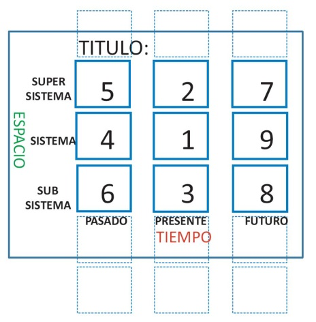
\includegraphics[scale=1.5]{imag/TRIZ.png}
\caption{Metodología de las nueva ventanas de TRIZ}
\label{1}
\end{figure}
\FloatBarrier






%-------------------------------------------------------------------------------------


\subsection{Marco Teórico}

\subsubsection{Fisioterapia Respiratoria}

Son procedimientos físicos utilizados en el tratamiento de pacientes con una incapacidad, enfermedad o lesión del aparato respiratorio, con el fin de alcanzar y mantener la rehabilitación funcional y evitar una disfunción, para este proyecto la idea principal es desarrollar un sistema que realice una técnica para rehabilitar la función pulmonar y prevenir complicaciones presentes en el paciente a tratar.


\subsubsection{Manejo de usuarios en Fisioterapia}

Los fisioterapias desempeñan roles de atención primaria para atender las necesidades de los pacientes, estos roles lo desempeñan en función de prestar  servicios de tratamiento respiratorio donde se puedan obtener resultados de los mismos, a partir de ello se deriva un modelo de manejo de pacientes estándar que contiene los elementos:  examen, evaluación, diagnostico, pronostico, intervención y respuestas 

\begin{figure}[ht]
\centering
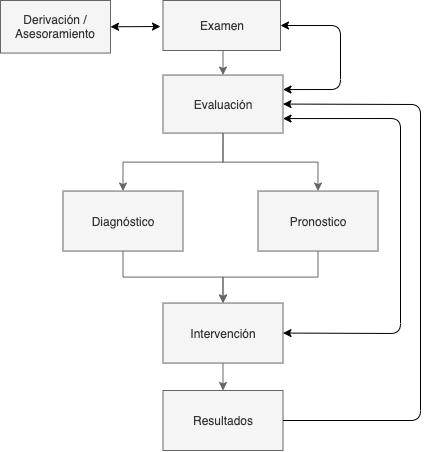
\includegraphics[scale=0.45]{imag/C4-Terapeuta.png}
\caption{Proceso de manejo de pacientes y usuarios por terapeuta. \textit{Guía para la práctica fisioterapéutica \cite{5}.}}
\label{2}
\end{figure}
\FloatBarrier





\subsubsection{Sesión de Fisioterapia}

Incluye los ejercicios, resultados, intervención y realimentación necesaria que un terapia de rehabilitación pulmonar de un paciente necesita.

\subsubsection{Ejercicios de Fisioterapia}

Las técnicas de re-expansión pulmonar son utilizadas por los fisioterapeutas para mejorar los volúmenes y capacidades pulmonares de los pacientes. Para entender las técnicas es importante conocer los volúmenes y capacidades pulmonares, como lo son(1)(2): 

\begin{itemize}
    \item Volumen de reserva inspiratoria (VIR) : volumen que se puede respirar después de una inspiración normal, 3000 ml.
    \item Volumen corriente (TV): volumen inspirado y espirado con cada respiración, 500 ml.
    \item Volumen de reserva espiratoria (ERV): volumen que puede expirar después de una respiración normal, 1100ml.
    \item Volumen residual (RV) : volumen que queda en el pulmón después de la espiración máxima (no se puede medir mediante espirometría), 1200ml.
    \item Capacidad inspiratoria (IC) : volumen que se puede respirar después de una exhalación normal, 3500 ml.
    \item Capacidad residual funcional (CRF) : volumen que queda en los pulmones después de la espiración normal, 2300 ml.
    \item Capacidad vital (VC) : volumen máximo que puede expirar después de la inspiración máxima, 4600 ml. 
    \item Capacidad pulmonar total (TLC) : volumen de aire en los pulmones después de la inspiración máxima, 6000 ml.
    
\end{itemize}


\begin{figure}[ht]
\centering
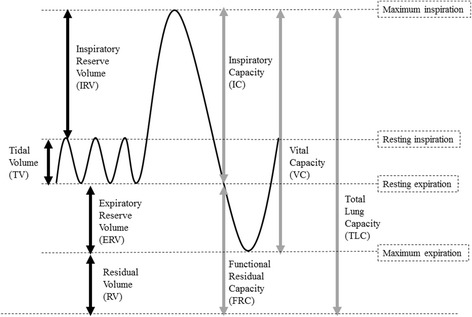
\includegraphics[scale=0.6]{imag/volumeslung.jpeg}
\caption{Medidas estándar de volumen pulmonar \cite{18}. }
\label{3}
\end{figure}
\FloatBarrier
















\subsubsection{Tratamiento de datos}

Monitorear la frecuencia respiratoria, volumen y saturación de oxigeno



\subsubsection{Historial clínico}


\subsubsection{Visualización de datos}

\subsubsection{Resultados de una Terapia Respiratoria}

Cada paciente o participante de una terapia respiratoria debe tener realimentación de los resultados 

%-------------------------------------------------------------------------------------


\section{Metodología de la investigación}

La metodología considerada para el desarrollo del proyecto es TRIZ que nos permite clasificar los atributos y características para definir los requerimientos del sistema inspirómetro integrado como define anteriormente, esta metodología se desarrolla en conjunto con el grupo de investigación de la Pontificia Universidad Javeriana Cali donde se integran áreas de fisioterapia, ingeniería de sistemas, ingeniería electrónica, diseño, ingeniería de software para desarrollar un sistema que permita realizar una terapia respiratoria y tenga realimentación visual para los usuarios, se plantea entonces los atributos del sistema en pasado, presente y futuro en nueve ventanas.

%fases de la metodología en diagrama

\subsection{Sistema presente} 

\subsubsection{Ventana 1}
En esta ventana se analizaron los diferentes elementos de ayuda para la recuperación pulmonar de un paciente con sistemas actuales, se identifica que estos sistemas siempre van acompañados de una terapia o denominada fisioterapia respiratoria, que como se explico anteriormente, es la encargada de definir que tipo de terapia es la mejor para cada complicación respiratoria.



\subsubsection{Ventana 2}

Se realiza el  análisis del supersistema, lo cual es en contexto donde se describen los elementos de ayuda para la recuperación de la capacidad pulmonar, en esta ventana se analizan las entidades o empresas que trabajan en la recuperación de la salud respiratoria, como también otros sectores relacionados con complicaciones respiratorias. 

En medicina, se utiliza respiración asistida en procesamientos quirúrgicos, donde se tienen en cuenta también técnicas respiratorias y fármacos para personas con enfermedades pulmonares. En industria, existen empresas que realizan el diseño y construcción de áreas limpias, manejo y control de ambientes hospitalarios y farmacéuticos. En lo social, esta directamente relacionado con el contagio de COVID por las personas que necesitan un tratamiento respiratorio asistido.

\subsubsection{Ventana 3}

Se realiza el  análisis del subsistema, donde se muestra de que están compuestos los diferentes elementos  investigados asociados a la recuperación de la capacidad pulmonar. Actualmente, se utilizan técnicas para la recuperación pulmonar de las personas, que se basan en una serie de instrucciones que el paciente debe seguir de acuerdo a la recomendación médica. Con un inspirómetro un paciente debe inhalar a través de la boquilla, lo que hace que la presión caiga dentro del dispositivo y, a su vez, hace que las bolas se eleven en cada uno de los tubos de flujo. Cada tubo está calibrado para que el desplazamiento completo de la pelota sea igual a un flujo específico, que se indica en la pared del tubo. El número de bolas y el nivel al que se elevan depende del nivel de flujo alcanzado. 

%https://patentimages.storage.googleapis.com/e3/b0/03/fefa9df55c113e/US20190134460A1.pdf

% investigar a nivel de software


Durante el análisis de la metodologías utilizadas en sistemas actuales, se identifica que una terapia respiratoria no se realiza adecuadamente debido a la falta de adherencia hacia la actividad por parte del paciente, además no existe un seguimiento con datos registrados que el terapeuta pueda evaluar, no hay un registro tampoco de un histórico de la evolución del paciente quien requiere principalmente indicaciones previas del terapeuta respiratorio.

\subsection{Sistema pasado}

\subsubsection{Ventana 4}

La rehabilitación pulmonar abarca desde los comienzos del arte médico, con ello, las principales estrategias utilizadas para disminuir el impacto de la enfermedad pulmonar crónica, las terapias recomendadas eran el reposo, evitar situaciones de esfuerzo físico o por el contrario entrenamientos físico con miras a rehabilitar los pacientes con el máximo posible de alcance de su sistema pulmonar y después de ello, también se desarrollaron técnicas aplicando los principios científicos entre los cuales vemos el entrenamiento muscular y oxígeno-terapia crónica domiciliaria.

\subsubsection{Ventana 5}

En el pasado no se tenía la conciencia de prevenir ciertos tipos de enfermedades como las respiratorias, de hecho no existían grandes compañías dedicadas al cuidado o rehabilitación de la capacidad pulmonar como las hay hoy en día. Solo existían esfuerzos e investigaciones individuales cuyas conclusiones permitieron que se desarrolle la industria que actualmente existe.

\subsubsection{Ventana 6}

Debido a que el pasado no existía una gran preocupación sobre enfermedades respiratorias y en general como las hay hoy en día, no había dispositivos que ayudaran a la recuperación pulmonar de las personas, salvo ejercicios de respiración que aún se usan en la fisioterapia respiratoria. 




\subsection{Sistema futuro} 

\subsubsection{Ventana 7}

En cuanto al futuro se entra al plano imaginario, en este caso el contexto en el que se encontraran los elementos de recuperación pulmonar. 
En medicina uno de los aspectos a mejorar es la de la reducción de tiempos de convalecencia en los hospitales porque minimiza costos tanto al hospital como al paciente además abre espacio para pacientes con otras patologías y una de las tendencias para lograr esto es la fisioterapia domiciliaria, que el paciente realice su terapia desde la comodidad de su casa y no tenga de desplazarse hasta el hospital. Desde lo social y ambiental, estos temas van de la mano debido a que en algunos países no se está trabajando lo suficiente en lo ambiental lo cual significa un aumento en la contaminación del aire que respiran las personas sobre todo en las grandes ciudades, lo cual también aumentaría la probabilidad de adquirir algunas afección respiratoria y sin tratamiento podría aumentar la tasa de mortalidad por estas causas. 

\subsubsection{Ventana 8}

El sistema ideado deberá usar algoritmos de programación para el envío y recepción de datos además de generar un reporte de datos de lo realizado por el paciente en el cual el profesional de la salud analizará el rendimiento del paciente.

\subsubsection{Ventana 9}

El software del inspirómetro deberá ser capaz de ejecutarse en el sistema operativo más usado en el mundo, con el fin de tener mayores posibilidades de uso.  Además deberá tener una interfaz gráfica intuitiva para que tanto el paciente como el terapeuta puedan usarlo de manera fácil y adecuada. Dicha interfaz deberá permitir modificar los límites de trabajo por parte del terapeuta con el fin de adaptar la terapia a los pacientes con mayores dificultades respiratorias. 


Dadas las características y atributos de los sistemas en pasado y presente, el sistema futuro, debe permitir que el paciente se pueda concentrar en su terapia y hacerla conscientemente, permitir adquirir datos, codificar, presentar y almacenar la información de desempeño de la terapia tanto al paciente como al terapeuta mediante una conexión remota, debe permitir la administración de usuarios, una plataforma con operaciones intuitivas para la programación de ejercicios para cada sesión y que permita la prescripción remoto de los mismos.

%-------------------------------------------------------------------------------------
\section{Proceso de Ingeniería de Software}



Bajo los atributos identificados con la metodología TRIZ se desarrollan a continuación los requerimientos funcionales y no funcionales del sistema software propuesto.


\subsection{Definición y especificación de requisitos}

En esta sección se detallan los procesos realizados para obtener los requisitos del sistema, la estructura y documentación de los requisitos, validación y priorización de estos.

\subsubsection{Diagrama de contexto}


\begin{figure}[ht]
\centering
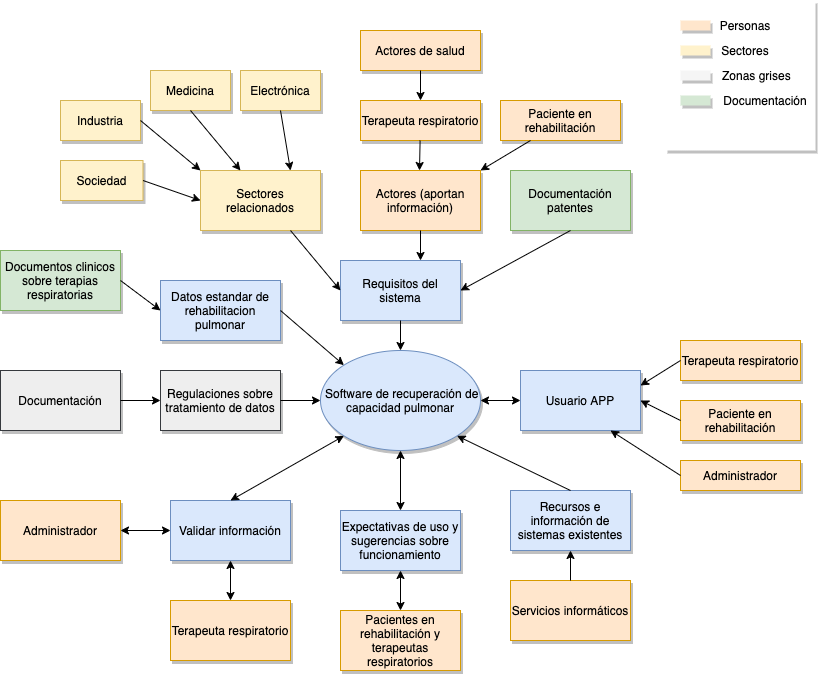
\includegraphics[scale=0.45]{imag/C4-Diagram contexto.png}
\caption{Diagrama de contexto de sistema software de capacidad pulmonar. }
\label{4}
\end{figure}
\FloatBarrier

\subsubsection{Técnicas de obtención de requisitos}

\begin{enumerate}
    \item \textbf{Reuniones grupales:} Inicialmente ser realizan reuniones grupales con los principales actores del sistema, tanto los posibles usuarios como terapeuta respiratorio como los desarrolladores del sistema de las diferentes áreas, software, electrónica y diseño
    \item \textbf{Encuestas:} 
        \begin{enumerate}
            \item Encuesta dirigida a fisioterapeutas tanto externos como internos del proyecto, con el propósito de identificar atributos comunes con los mencionados en el grupo de investigación, para lograr el objetivo, se realizaron preguntas orientadas a las terapias respiratorias, los datos que se evalúan actualmente y las metodologías utilizadas.
            \item Encuesta dirigida a los pacientes con el fin de conocer la experiencia de los pacientes que han realizado terapia respiratoria con el inspirómetro incentivo en cuanto a la terapia y el acompañamiento con el terapeuta.
        \end{enumerate}
    
    
\end{enumerate}




\subsubsection{Definición de requisitos funcionales}

%Modulo Fisioterapeuta============================================ 

 % FUNCIÓN EVALUAR
\begin{enumerate}[start=1,label={\bfseries RF0\arabic*.}]

    \item El sistema debe tener una funcionalidad para el terapeuta respiratorio que le permita evaluar el estado de un paciente para poder realizar un diagnostico y posteriormente recetar la terapia correspondiente por paciente, si es necesario.
        \label{RF01}
            \begin{enumerate}[label*=\arabic*.]
                \item La funcionalidad para el terapeuta respiratorio debe permitirle evaluar las sesiones realizadas por paciente.
                
                \item La funcionalidad para el terapeuta respiratorio debe permitirle la visualización de datos como flujo, frecuencia, volumen respiratorio y saturación de oxigeno por cada sesión por medio de gráficas de desempeño.
                
                \item La funcionalidad para el terapeuta respiratorio debe permitirle revisar la evolución del paciente dados los datos de flujo, frecuencia, volumen respiratorio y saturación de oxigeno.  %de las terapias por sesion
                
                \item La funcionalidad para al terapeuta respiratorio debe permitirle ver estadísticas de las terapias realizadas y del uso de la aplicación por los pacientes. %TABLAS?
                
              
            \end{enumerate}

    %EJERCICIOS     --como quedan descritos? animaciones, textos ?
    \item El sistema debe tener una funcionalidad para el terapeuta respiratorio que le permita programar  ejercicios por cada sesión en la aplicación.
        
        \label{RF02}
            \begin{enumerate}[label*=\arabic*.]
            
                \item La funcionalidad de programar ejercicios para el terapeuta respiratorio que le permita cargar de ejercicios definidos en texto con sus tareas correspondientes. %completar si son descritos, texto o con animaciones
                 
                \item La funcionalidad de programar ejercicios para el terapeuta respiratorio debe tener una funcionalidad para al terapeuta respiratorio que le permita el almacenamiento de ejercicios prescritos. %completar
                
                \item La funcionalidad de programar ejercicios para el terapeuta respiratorio debe permitir modificar los ejercicios, cargar o eliminar tareas prescritas
                
                \item La funcionalidad de programar ejercicios para el terapeuta respiratorio debe permitir establecer parámetros de ejercicios por conexión remota
     
     
                
            \end{enumerate}
            
    %ORIENTAR
    \item  El sistema debe tener una funcionalidad para al terapeuta respiratorio que le permita orientarse ya sea en el uso de la aplicación, como en el manejo de los ejercicios establecidos.
    
    \label{RF03}
            \begin{enumerate}[label*=\arabic*.]
                %Posible requerimiento
                \item La funcionalidad para al terapeuta respiratorio debe permitir notificar los ejercicios tanto los que se han realizado como los que no han sido realizados por los pacientes. 
                
                \item La funcionalidad para al terapeuta respiratorio debe incluir una guía de usuario que especifique una secuencia para usar la aplicación correctamente. %completar
            \end{enumerate}
            
    
    %PACIENTES
    \item  El sistema debe tener una funcionalidad para al terapeuta respiratorio que le permita la gestión de los parámetros de cada sesión por medio de los perfiles de cada paciente, parámetros tales como  el rango de medición de flujo inspirado, volumen, frecuencia respiratoria y saturación de oxigeno por cada paciente. %preguntar       
    \label{RF04}
            \begin{enumerate}[label*=\arabic*.]
                \item La funcionalidad de gestión de parámetros que le permita al terapeuta establecer rangos en volumen, frecuencia y saturación de oxigeno por medio de teleconsulta. %videollamada?
                
                \item La funcionalidad para al terapeuta respiratorio debe permitir establecer parámetros de flujo inspirado y asignar los ejercicios correspondientes por paciente
                
                
            \end{enumerate}
            
    %DIAGNOSTICO
    \item El sistema debe tener una funcionalidad para al terapeuta respiratorio que le permita realizar un diagnostico dados los datos del paciente.%completar
    
    \item  El sistema debe tener una funcionalidad de envió de vídeos para brindar realimentaciones de manera cualitativa e instrucciones necesarias para la terapia.
    
    
    %ALMACENAR DATOS
    \item El sistema debe tener una funcionalidad para al terapeuta respiratorio que le permita guardar los cambios realizados en la plataforma ya sea en modificaciones de las sesiones o pacientes.
    
    
    
            
%Modulo Paciente===================================================================

 %ORIENTAR
    \item El sistema debe tener una funcionalidad que permita orientar al paciente  para la realización de un ejercicio de una terapia respiratoria. 
    \label{RF08}
            \begin{enumerate}[label*=\arabic*.]
            
                \item La funcionalidad de orientar al paciente debe incluir una demostración con los pasos o secuencia a seguir sobre como manejar la aplicación, como usar el inspirómetro electrónico y como realizar el ejercicio prescrito.
                
                \item La funcionalidad de orientar al paciente de manera sensitiva debe permitir generar una secuencia en la terapia por cada sesión establecida al paciente, los ejercicios permitirán el estimulo que el paciente  necesita para su recuperación. %que serían las cualidades de la orientación
                
                \item La funcionalidad de orientar al paciente debe contar con una guía de usuario que debe incluir una demostración con los pasos o secuencia a seguir sobre como manejar la aplicación.
                
                \item La funcionalidad de orientar al paciente debe contar con un realimentación después de una sesión realizada que permita dar a conocer resultados y consejos de avance en terapia para una próxima sesión, esta funcionalidad se dará con la intervención del terapeuta al finalizar cada sesión.
    
                \item La funcionalidad de orientar al paciente debe mostrar datos de evolución que permitan conocer el estado en que se encuentra el paciente para completar una terapia respiratoria.
                
                \item La funcionalidad de orientar al paciente debe contar con una guía sobre como usar el inspirómetro electrónico y como realizar el ejercicio prescrito, resaltando también los limites de seguridad del sistema.
            \end{enumerate}
            
            
        %enviar realimentacion por otros medios no solo visual

%Modulo de  Administración============================================    

 
    \item El sistema debe contar con una estructura de gestión de usuarios.
    %Grupos de pacientes  
    \item El sistema debe permitir a los terapeutas  administrar grupos de pacientes para asignar las respectivas sesiones.
    \label{RF10}
        \begin{enumerate}[label*=\arabic*.]
            \item La funcionalidad de grupo de pacientes debe permitir a los terapeutas la creación y administración de grupos de pacientes, los cuales van a tener en su plataforma registrados con los datos demográficos de cada paciente.
            
            \item La funcionalidad de grupo de pacientes debe permitir a los terapeutas asignar terapias o en los que se puedan definir la fecha de inicio y la duración máxima por cronómetro para realizar cada actividad para este caso el terapeuta debe seleccionar y asignar una actividad previamente.
        \end{enumerate}
        
    \item El sistema debe mostrar información personalizada para cada usuario
            
 
     
         
    
%Modulo sistema central de procesamiento===========================================
 
    
    %Adquirir datos
    
    \item El sistema debe permitir Adquirir, presentar y almacenar los datos del desempeño y seguimiento de la terapia (i.e. cuánto le falta, cuánto avanzó) al fisioterapeuta y al paciente por conexión remota.
     \label{RF12}
            \begin{enumerate}[label*=\arabic*.]
                
                \item El sistema debe tener una funcionalidad de toma de datos del paciente que permita agrupar la captura de datos en un historial con datos del paciente, que registre los datos de flujo, frecuencia respiratoria por cada sesión 
                
                \item La funcionalidad de toma de datos del paciente debe permitir hacer el registro de datos mediante un método cuantitativo de grabación de datos. Mediante los estímulos capturados uno a uno desde el inspirómetro %evaluar
                
                \item La funcionalidad de codificar la variable física medida a partir de los datos derivados del flujo respiratorio, frecuencia respirato %Codificar la información de la variable física medida. (estructura de datos)
            
            \end{enumerate}
            
    \item La funcionalidad de toma de datos del paciente debe permitir hacer el registro de datos mediante un método cuantitativo de grabación de datos.
            
    %Tratamiento de datos
        
    \item El sistema debe encargarse de la conversión de datos que recibe desde el inspirómetro, presentarlos en volumen y frecuencia estimados de un ejercicio realizado por el paciente.
       

    
    %Trasmisión de datos
    
    \item El sistema debe contar con una API para permitir la trasmisión de datos.
    
   
    
    %Almacenamiento de datos
    
   
    \item La funcionalidad de toma de datos del paciente debe garantizar el auto-guardado por cada actividad realizada.
    
    \item El sistema debe permitir estructurar los datos y mostrarlos en tablas de frecuencia.
    
    \item El sistema debe permitir almacenar la información adquirida de manera local proveniente de los ejercicios de fisioterapia, debe contar con capacidad de memoria a partir de un formato estándar de memoria.
    
    \item El sistema debe permitir almacenar los datos adquiridos de la medición de flujo inspirado proveniente del inspirómetro de manera local.
    
  
    
    
    %Gamificación
    \item El sistema debe permitir integrar un modulo de gamificación que permitira acoplarse con el sistema de ejercicios para programar por el usuario terapeuta.
    
     
    
    %%Juego
    \item El sistema debe permitir mantener un flujo y volumen respiratorio constante indicado en los ejercicios prescritos por el terapeuta.
    %porque eso le va a permitir que el flujo de aire llegue a los alveolos y realice el íntercambio, La parte de ser constante y laminar hace que la bolita o lo que se mira en el incentivo, Este quieta en un solo lugar, Sin subir o bajar,Entonces esa bolita quieta y a la altura  me permite saber que si lo esta haciendo bien, Si, pues dependiendo del volumen a donde el profesional le indique a la persona llegar. Ya que el dispositivo tiene aun lado marcado como en rayitas los niveles de volumen que se esta alcanzando
    \label{RF21}
            \begin{enumerate}[label*=\arabic*.]
                \item La funcionalidad de mantener un flujo y volumen constante en cada ejercicio deber permitir identificar si el paciente esta siguiendo los pasos indicados en el ejercicio.%preguntar
                \item La funcionalidad de mantener un flujo y volumen constante en cada ejercicio deber permitir registrar los niveles de volumen y frecuencia respiratoria 
            \end{enumerate}
    
        

%https://www.gloomaps.com/3zr2f3aYfo

\end{enumerate}


\subsubsection{Definición de requisitos no funcionales}

\begin{enumerate}[start=1,label={\bfseries RNF\arabic*.}]


\item  El sistema no debe ser exigente en tecnología para que pueda ser usado por cualquier paciente con un sistema tecnológico de comunicación. %Android

\item El sistema debe estar en la capacidad de funcionar en modo offline, es decir soporte sin conexión, cuando las condiciones de conexión con el servidor sean adversas, asegurando que la información no se pierda a causa de estos imprevistos

\item El sistema debe permitir que cualquier usuario que no conozca a profundidad el funcionamiento de las TIC tenga un buen desempeño con el manejo de la herramienta

\item El sistema debe asegurar una disponibilidad del 99.0 \%

\item El sistema debe ser desarrollado bajo los principios de diseño SOLID

\item El sistema debe tener un tiempo TTI menor o igual a 5 segundos

 \item El sistema debe cumplir con parámetros ACID para el relacionamiento con bases de datos
 
\item El sistema debe contar con las características necesarias para hacer un deploy sencillo

\item El sistema debe contar con una función de backup y de recuperación ante fallos
\item El sistema debe soportar concurrencia de múltiples usuarios
\item El sistema debe contar con los protocolos necesarios para asegurar un funcionamiento seguro a través de Internet, es decir, que la información enviada y recibida este protegida contra ataques de robo información y suplantación de identidad. 
\item El sistema no debería ser invasivo.
        
\item El sistema debe favorecer la adherencia al tratamiento de fisioterapia.

\end{enumerate}




\subsubsection{Definición de requisitos tipo restricción}

\begin{enumerate}[start=1,label={\bfseries RTR\arabic*.}]

\item Poner el mínimo número de comandos de operación para el paciente.


\end{enumerate}

%-------------------------------------------------------------------------------------





\newpage


\subsection{Arquitectura del sistema}

%C1

Dados las especificaciones de los servicios de terapia respiratoria y los requerimientos desarrollados se construye la siguiente arquitectura del sistema

\begin{figure}[ht]
\centering
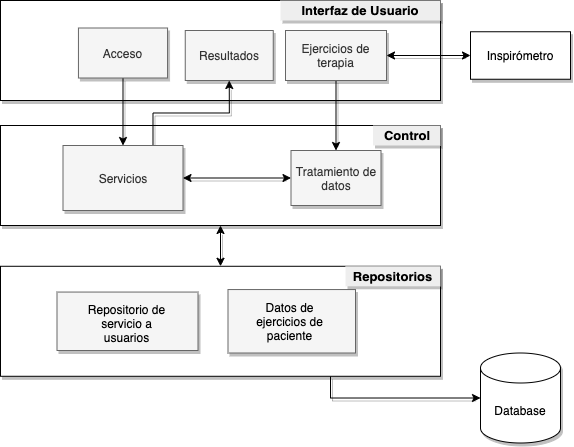
\includegraphics[scale=0.5]{imag/C4-Sistema1.png}
\caption{Arquitectura de primer nivel del sistema de terapia respiratoria}
\label{5}
\end{figure}
\FloatBarrier

Se identifican funcionalidades especificas del sistema y se separan los servicios:

%C2


\begin{figure}[ht]
\centering
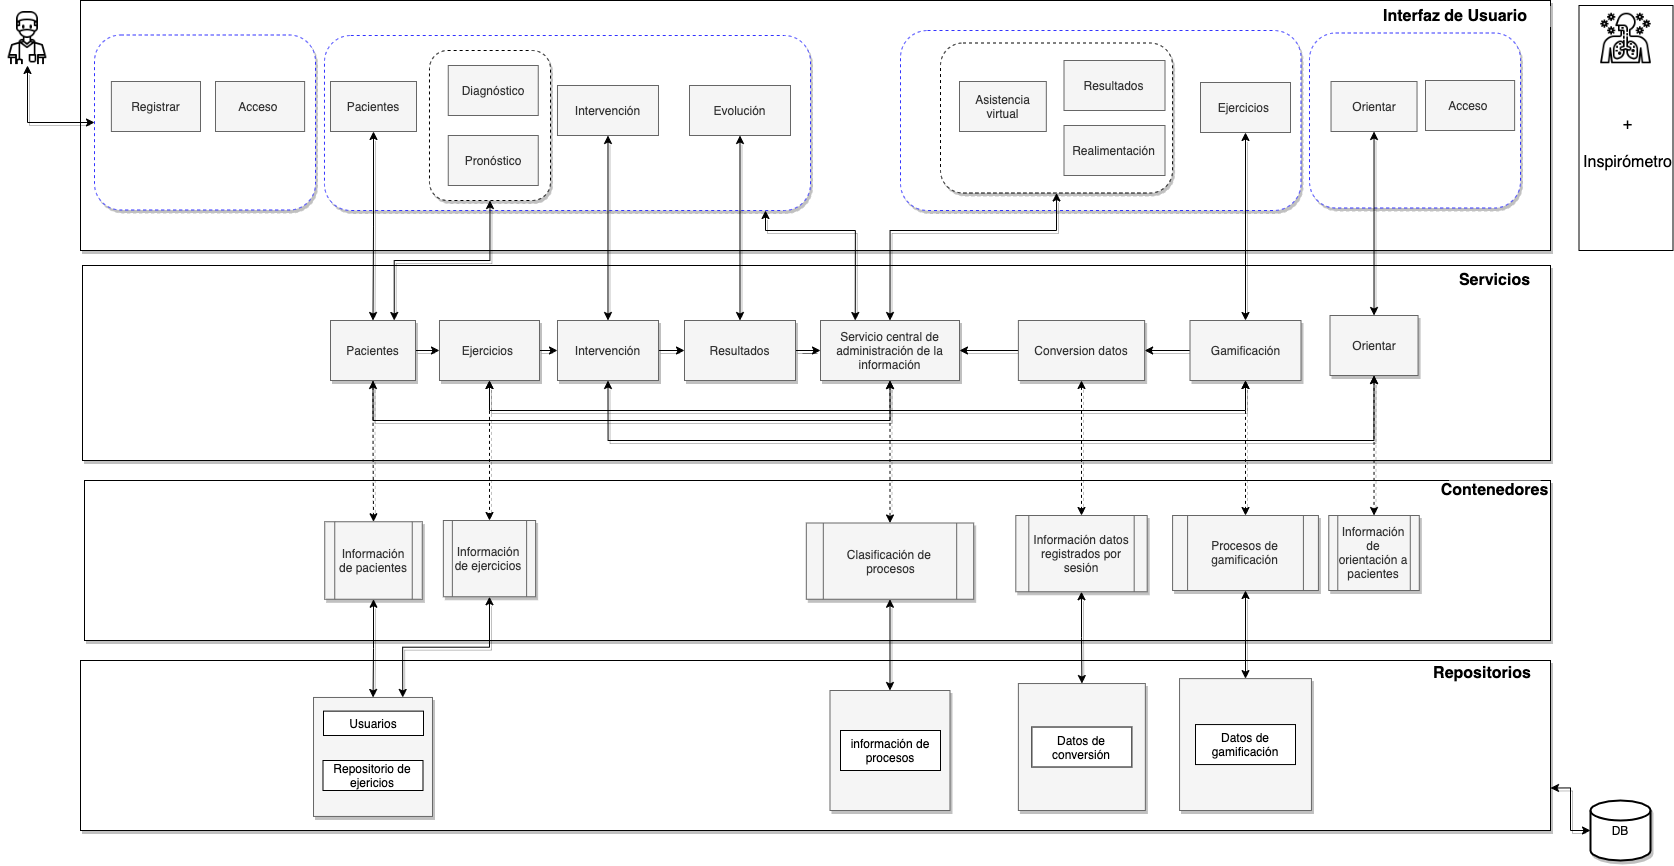
\includegraphics[scale=0.25]{imag/C4-Nivel2.png}
\caption{Arquitectura de segundo nivel del sistema de terapia respiratoria}
\label{6}
\end{figure}
\FloatBarrier


%C3


%C4




\section{Desarrollo del Sistema}

\section{Análisis de Resultados}

\subsection{Análisis estadístico de datos}





%-------------------------------------------------------------------------------------
\section{Conclusiones y recomendaciones}


\section{Trabajos Futuros}




\newpage



%%%%%%%%%%%%%%%%%%%%%%%%%%%%%
% BIBLIOGRAFIA
%%%%%%%%%%%%%%%%%%%%%%%%%%%%%
\bibliography{biblio.bib}
\bibliographystyle{IEEEtran}
\nocite{1}
\nocite{2}
\nocite{3}
\nocite{4}
\nocite{5}

%%%%%%%%%%%%%%%%
% GENERAL INDEX
%%%%%%%%%%%%%%%%
%\printindex



\section{Anexos}




\end{document}


